%%%%%%%%%%%%%%%%%%%%%%%%%%%%%%%%%%%%%%%%%%%%%%%%%%%
%% P3: Phenomenology of Particle Physics                         
%%
%% Author:  André Rubbia                   		 
%%
%% Figure 28.13 Total neutrino and antineutrino cross-sections for different types of reactions as a function of  energy.
%%
%% This work is licensed under the Creative Commons Attribution 4.0 International License. 
%% To view a copy of this license, visit http://creativecommons.org/licenses/by/4.0/ or 
%% send a letter to Creative Commons, PO Box 1866, Mountain View, CA 94042, USA.
%%
%%%%%%%%%%%%%%%%%%%%%%%%%%%%%%%%%%%%%%%%%%%%%%%%%%%

\documentclass[a4paper,10pt]{article}

\usepackage[T1]{fontenc}
\usepackage[utf8]{inputenc}
\usepackage{lmodern}
\usepackage[labelfont=bf]{caption}
\usepackage{upgreek}

\usepackage{amssymb}
\usepackage{amsmath}
\usepackage{mathtools}

\usepackage{tikz}
\usepackage{pgfplots}
\pgfplotsset{compat=1.17}
\usepgfplotslibrary{ternary}
\usepgfplotslibrary{fillbetween}
\usepgfplotslibrary{external}

\def\d{\mathrm{d}}
\setlength{\oddsidemargin}{-1.0cm}
\setlength{\evensidemargin}{-1.0cm}
\setlength{\textheight}{25cm}
\setlength{\textwidth}{18cm}

\pgfkeys{/pgf/number format/.cd,1000 sep={}}

\begin{document}

%%%%%%%%%%%%%%%%   FIGURE  %%%%%%%%%%%%%%%%%%%%%%%%%%%%%%
\begin{figure}[htbp]
\begin{center}
\begin{tikzpicture}[scale=1]
\begin{loglogaxis}[
    title={Total neutrino cross-section},
    xlabel={Neutrino energy (GeV)},
    ylabel={$\sigma_{tot}$ (cm$^2$)},
    height=0.7\textwidth,
    width=0.9\textwidth,
    xmin=0.1, xmax=1e3,
    ymin=1e-42, ymax=1e-34,
    legend pos=north west,
		legend columns=2,
    ymajorgrids=true,
    xmajorgrids=true,
   grid style=dashed,
]
    \legend{$\nu_\mu N\rightarrow \mu^-X$ (CC DIS),
    $\bar \nu_\mu N\rightarrow \mu^+X$ (CC DIS),
    $\nu_\mu N\rightarrow \nu_\mu X$ (NC DIS),
    $\bar \nu_\mu N\rightarrow \bar\nu_\mu X$ (NC DIS),
		$\nu_\mu n\rightarrow \mu^-p$ (QE),
		$\bar\nu_\mu p\rightarrow \mu^+n$ (QE),
    $\nu_\mu e \rightarrow \mu^- \nu_e$ (IMD),
    $\nu_e e \rightarrow \nu_e e$,
    $\bar \nu_e e \rightarrow \bar \nu_e e$,
    $\nu_x e \rightarrow \nu_x e$,
    $\bar \nu_x e \rightarrow \bar \nu_x e$
    }
    	\addplot[domain=1:1e3,blue,very thick] {0.677e-38*x};
    	\addplot[domain=1:1e3,magenta,very thick] {0.334e-38*x};
    	\addplot[domain=5:1e3,blue,dashed, very thick] {0.31*0.677e-38*x};
    	\addplot[domain=5:1e3,magenta,dashed, very thick] {0.38*0.334e-38*x};
	% quasi elastic from NUX generator
			\addplot[very thick] coordinates {
			(    0.1259,0.5025E-39)
			(    0.1585,0.1268E-38)
			(    0.1995,0.2315E-38)
			(    0.2512,0.3610E-38)
			(    0.3162,0.5165E-38)
			(    0.3981,0.6770E-38)
			(    0.5012,0.8302E-38)
			(    0.6310,0.9497E-38)
			(    0.7943,0.1031E-37)
			(    1.0000,0.1075E-37)
			(    1.2589,0.1089E-37)
			(    1.5849,0.1084E-37)
			(    1.9953,0.1070E-37)
			(    2.5119,0.1052E-37)
			(    3.1623,0.1034E-37)
			(    3.9811,0.1018E-37)
			(    5.0119,0.1004E-37)
			(    6.3096,0.9930E-38)
			(    7.9433,0.9836E-38)
			(   10.0000,0.9761E-38)
			(   12.5893,0.9701E-38)
			(   15.8489,0.9653E-38)
			(   19.9526,0.9615E-38)
			(   25.1189,0.9585E-38)
			(   31.6228,0.9561E-38)
			(   39.8107,0.9542E-38)
			(   50.1187,0.9527E-38)
			(   63.0957,0.9516E-38)
			(   79.4328,0.9505E-38)
			(  100.0000,0.9498E-38)
			(  125.8925,0.9493E-38)
			(  158.4893,0.9487E-38)
			(  199.5262,0.9483E-38)
			(  251.1887,0.9481E-38)
			(  316.2278,0.9478E-38)
			(  398.1071,0.9476E-38)
			(  501.1873,0.9476E-38)
			(  630.9573,0.9473E-38)
			(  794.3284,0.9472E-38)
			( 1000.0000,0.9473E-38)
};
% quasi elastic from nux
		\addplot[very thick, dashed] coordinates {
		(    0.1259,0.2686E-39)
		(    0.1585,0.5129E-39)
		(    0.1995,0.7385E-39)
		(    0.2512,0.9450E-39)
		(    0.3162,0.1177E-38)
		(    0.3981,0.1485E-38)
		(    0.5012,0.1848E-38)
		(    0.6310,0.2265E-38)
		(    0.7943,0.2719E-38)
		(    1.0000,0.3306E-38)
		(    1.2589,0.3842E-38)
		(    1.5849,0.4378E-38)
		(    1.9953,0.4864E-38)
		(    2.5119,0.5371E-38)
		(    3.1623,0.5719E-38)
		(    3.9811,0.6100E-38)
		(    5.0119,0.6387E-38)
		(    6.3096,0.6662E-38)
		(    7.9433,0.6897E-38)
		(   10.0000,0.7006E-38)
		(   12.5893,0.7293E-38)
		(   15.8489,0.7512E-38)
		(   19.9526,0.7427E-38)
		(   25.1189,0.7636E-38)
		(   31.6228,0.7371E-38)
		(   39.8107,0.8050E-38)
		(   50.1187,0.7817E-38)
		(   63.0957,0.7515E-38)
		(   79.4328,0.8167E-38)
		(  100.0000,0.7910E-38)
		(  125.8925,0.7591E-38)
		(  158.4893,0.8228E-38)
		(  199.5262,0.7959E-38)
		(  251.1887,0.7631E-38)
		(  316.2278,0.8259E-38)
		(  398.1071,0.7986E-38)
		(  501.1873,0.7653E-38)
		(  630.9573,0.8277E-38)
		(  794.3284,0.8000E-38)
		( 1000.0000,0.7666E-38)
};

% IMD,
    	\addplot[domain=11:1e3,brown, very thick,samples=100] {0.389e-31*1e4*(1.16e-5)^2*(2*0.511e-3*x-0.105^2)^2/3.1415/(2*0.511e-3*x)};
% sigma^0 = 1.720e-41 Enu cm^2
    	\addplot[domain=0.1:1e3,cyan,very thick] {1.72e-41*((1-0.27)^2+(0.23^2)/3)*x};
    	\addplot[domain=0.1:1e3,red,very thick] {1.72e-41*((0.23)^2+((1-0.27)^2)/3)*x};
    	\addplot[domain=0.1:1e3,dashed,cyan,very thick] {1.72e-41*((-0.27)^2+(0.23^2)/3)*x};
    	\addplot[domain=0.1:1e3,dashed,red,very thick] {1.72e-41*((0.23)^2+((-0.27)^2)/3)*x};
%
    	\addplot[domain=0.5:1,blue,dotted, very thick] {0.677e-38*x};
    	\addplot[domain=0.5:1,magenta,dotted, very thick] {0.334e-38*x};
\end{loglogaxis}
\end{tikzpicture}
\caption{Total neutrino and antineutrino cross-sections for different types of reactions
as a function of  energy.}
\end{center}
\end{figure}
%
%%%%%%%%%%%%%%%%   END FIGURE  %%%%%%%%%%%%%%%%%%%%%%%%%%%%%%
%


\end{document}
